% Put labels, etc., on figures using PSTricks.
% Use dvips -E <file>.dvi -o <file>.eps to create encapsulated PostScript.
% Use epstool --copy --bbox <file>.eps <new_file>.eps to fix problems with bounding box.
\documentclass[12pt]{article}
\usepackage{graphicx}
\usepackage{pstricks}
\pagestyle{empty}

\begin{document}
\rput(5,-5){
\rput{L}(.1,-.1){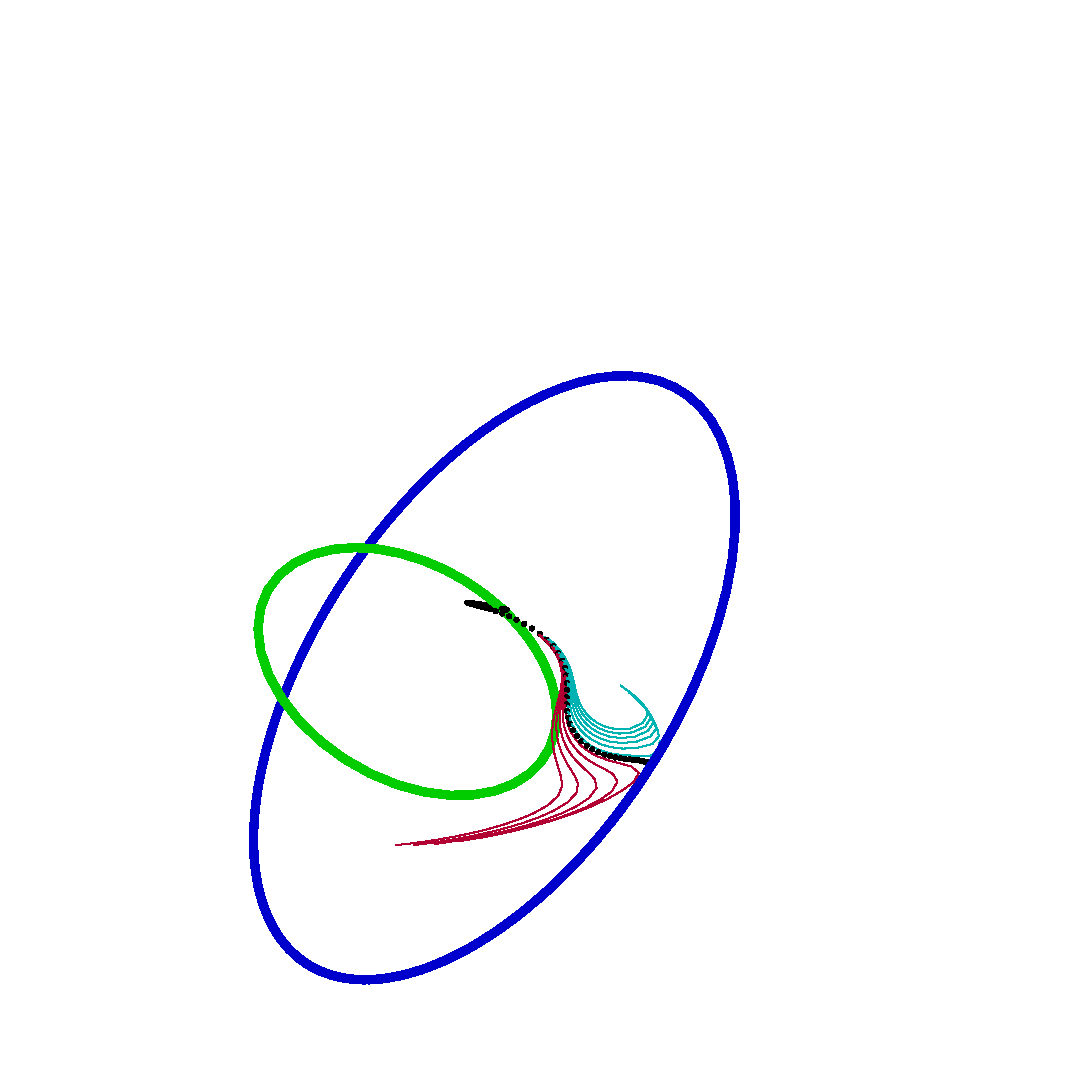
\includegraphics{../../rpo_ks/figs_pst/splitting.eps}}

\huge

\psframe*[linecolor=white](-6.5,6)(-5.5,7)
\psframe*[linecolor=white](6,-6.5)(7.2,-5.5)

\rput(6.5,0.5){E$_3$} 

\rput(-0.5,-4){E$_2$}



% Use grid command below to place objects at specified coordinates.
%\psgrid[subgriddiv=1,griddots=10](-8,-8)(10,10)
}
\end{document}
